% LTeX: language=en-GB
\chapter{Methodology: the Airbag Design Workflow}
\label{chapter:methodology}


\section{Problem statement}
To properly outline and, more importantly, test the workflow proposed as a main objective of this thesis, it is necessary to identify the specific context in which this project is embedded, as it originates from prior research work conducted within the specific framework of Turin. The design inputs presented below were gathered from analysing the results presented by the group (\cite{Cavallo2020}, \cite{Bertelli2021}, \cite{Sivieri2021}, \cite{Fiorentino2021}, and \cite{Angelini2023}) and categorising them into mission aspects on which to root the proposal of Section \ref{section:proposed-approach}.

\subsection{Reference mission and design inputs}
\subsubsection{Route and flight profile}
The reference mission is based on a hospital-to-hospital route as initially suggested by Cavallo (2020) \cite{Cavallo2020}, connecting two hospitals across the city of Turin as shown in Fig. \ref{fig:trajectory-map}, representing a city map with route schematics. In particular, the starting point is the Molinette Hospital in the southern region of the city, and the destination is the San Giovanni Bosco hospital in the northern sector. As they are located far apart, these two hospitals require medical deliveries to traverse a broad part of the city's territory. The hospitals are connected through two possible routes:
\begin{itemize}
    \item \textbf{Route A}: Initially hypothesised by Cavallo and confirmed by Bertelli (2021) \cite{Bertelli2021}, it takes advantage of the above-water air corridor over the river Po and its tributary Stura, mostly skirting the city and flying over city ground only in the relatively short segments connecting the hospitals to the rivers. Among the two routes, it is the safest (and, thus, most certifiable according to Cavallo) as it reduces the probability of ground impact in case of drone failure due to the UAV's permanence in the above-water air corridor. This route was selected as viable within the Concept of Operations (ConOps) that informed the preliminary drafting of the SORA. Approximate length: 10\,km. Approximate duration time: 15\,min, comparable to ambulance-based delivery times.
    \item \textbf{Route B}: A crude alternative to Cavallo and Bertelli's Route A, connecting the two hospitals in a straight line over the city. Angelini (2023) \cite{Angelini2023} deemed this route infeasible based on their comparative safety analysis of delivery means, primarily due to the lack of proper risk mitigation measures concerning in-flight failures. However, as the approach proposed in this thesis aims at partially mitigating these risks, it was chosen to consider this route (at least for preliminary evaluation).
    \item \textbf{Alternative routes \textit{(omitted from analysis)}}: Fiorentino (2021) \cite{Fiorentino2021} and Angelini (2024)'s \cite{Angelini2023} work is rooted in minimum risk-based route selection considering territories that extend beyond city borders, specifically including the entire province\footnote{In Italy, local government is organised across three administrative levels: regions, provinces, and municipalities. Here, assessing the Province of Turin corresponds to evaluating the territorial sub-region of Piedmont administered by the provincial capital of Turin.} in case of Angelini's study. Either using the RRT* algorithm in Fiorentino's case or the Dijkstra and A* algorithms in Angelini's case, these two studies share a common approach of considering multiple layers (\hl{such as population density, shelters, and critical infrastructure CHECK}) to calculate the probabilistic minimum-risk paths for different means of transportation (eVTOL, UAV, etc.), without predefined start and end points, thereby determining the optimal drone hub location across the province. \hl{valid for FIORENTINO TOO???} The results of these works were omitted from the definition of the reference mission for two main reasons. First, they do not specifically target hospital-to-hospital operations; their scope focuses on optimising general logistics rather than facilitating inter-hospital transport, contrarily to one of the primary objectives of the present thesis. Second, their findings indicate that drone operations, when evaluated against the merit indices adopted in their analyses, are deemed unviable due to safety constraints. In contrast, the objective of this research is precisely to identify a mission scenario that is unfeasible under current conditions and implement risk-mitigation strategies to ultimately enable drone transit.
\end{itemize}


In either Route A or B, as specified in Bertelli's ConOps, the cruising height is about 75\,m, at 17\,m/s cruising velocity (approximately 70\% of the maximum cruising speed allowed by the UAV platform of 25\,m/s, unsustainable for the entire duration of the mission at the time of evaluation), with possible speed variations according to mission urgency if specified in the ConOps. 

Accounting for the presence of wind in the operating environment, wind speed in Turin averages about 1.8\,m/s (6.5\,km/h) \cite{ComuneTorinoWind-AVG}, with a peak of about 28.6\,m/s (103\,km/h) in 2013 \cite{ComuneTorinoWind-MAX}.

\begin{figure}[h!]
    \centering
    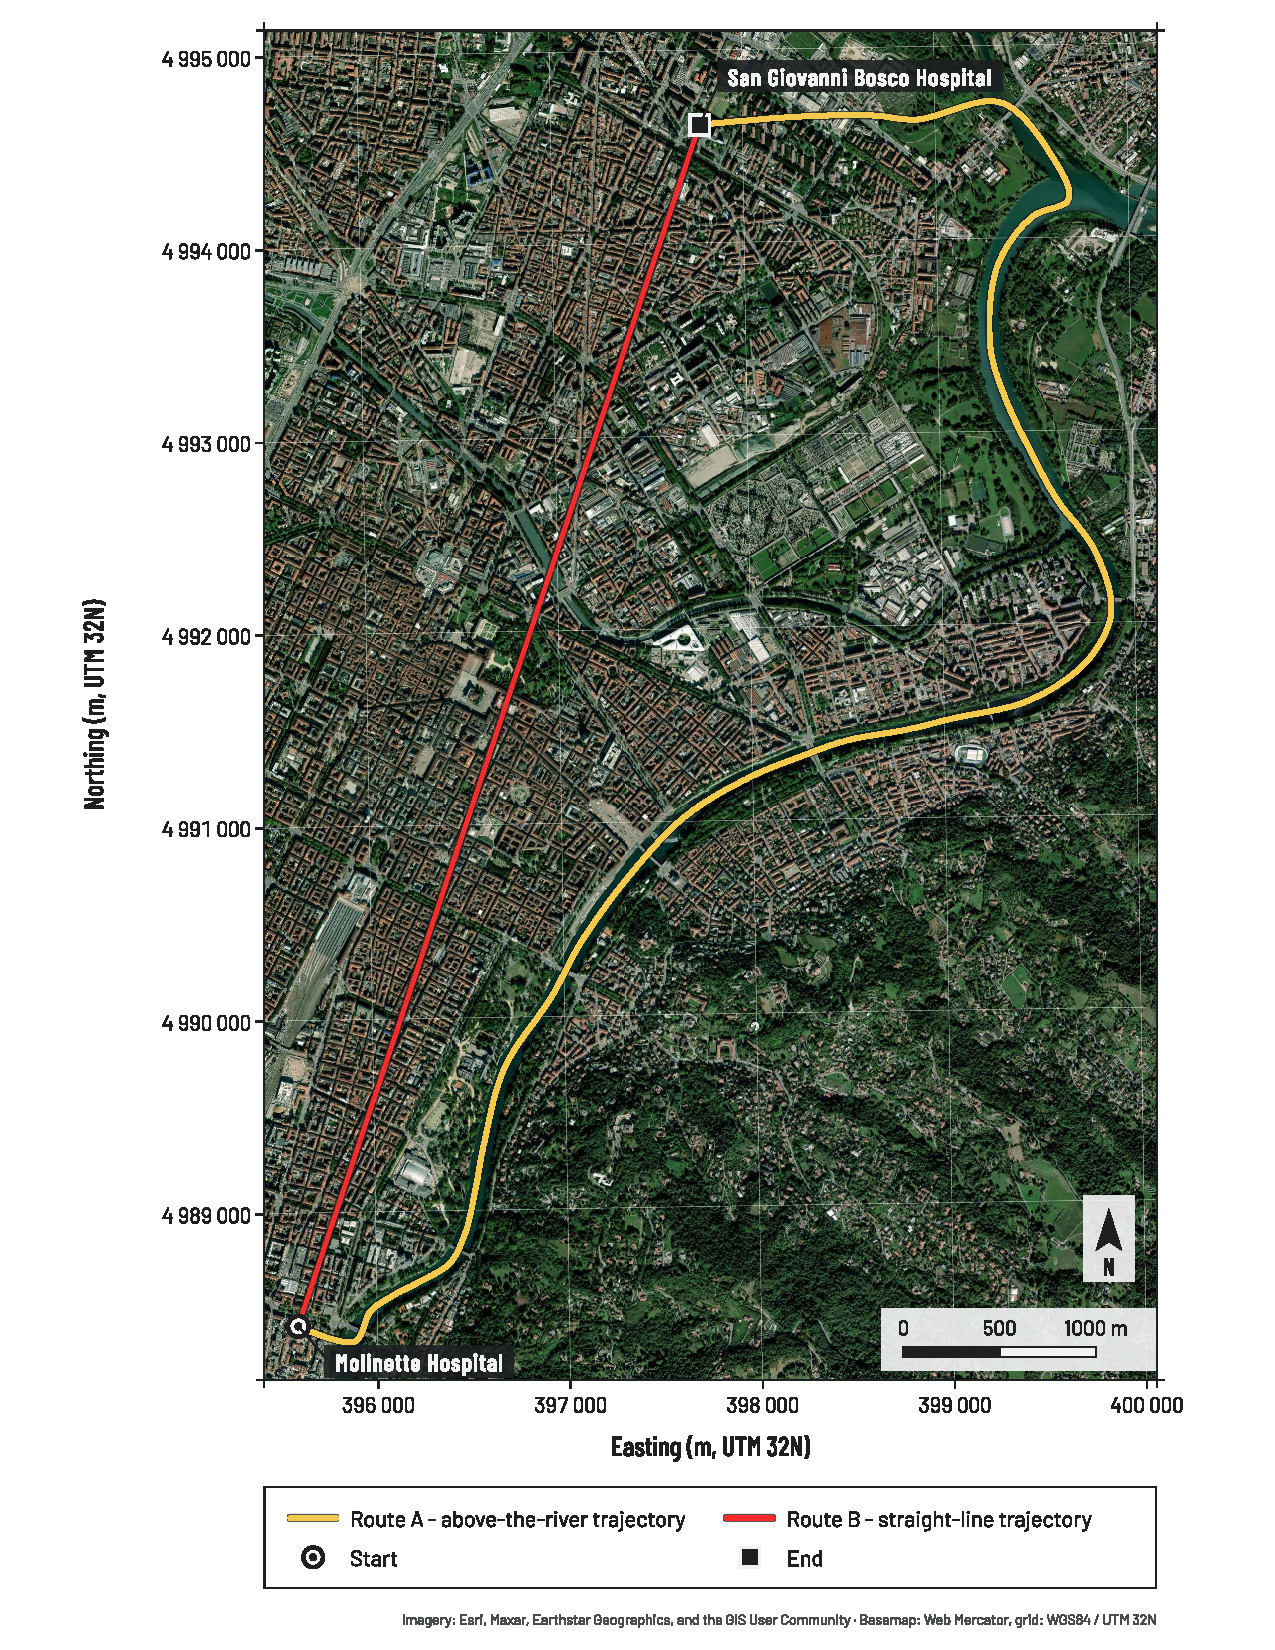
\includegraphics[height=0.54\textheight, keepaspectratio, trim=35 24 41 7, clip]{figures/chap3/trajectory-map-satellite.pdf}
    \caption[Reference mission routes across Turin]{Reference mission routes across Turin, from the Molinette Hospital to the San Giovanni Bosco Hospital: Route A (above-the-river trajectory) and Route B (straight-line trajectory).\protect\footnotemark}
    \label{fig:trajectory-map}
\end{figure}
\footnotetext{Imagery: Esri, Maxar, Earthstar Geographics, and the GIS User Community. Basemap: Web Mercator; grid: WGS84 / UTM 32N.}


\subsubsection{UAV Platform}
The UAV platform choice is inherently linked to the reference mission specifications above, meaning that the platform is required to sustain the cruising speed requirements specified in the ConOps. A Maximum Takeoff Mass (MTOM) of 9\,kg and a 0.81\,m characteristic dimension were also specified in Bertelli's ConOps, leading to the suggestion of a potential drone model suitable for the situation: DJI's \textit{Matrice 300 RTK}. Despite having characteristics suitable for the speed requirements, the drone has a payload limit of 2.7\,kg and a wind resistance of 15\,m/s in cruise. While this drone was initially selected for the preliminary SORA, its specific parameters are not binding for the present study. In particular, the payload-mass and wind-resistance limitations may be disregarded, given that the ConOps set a much broader requirement for MTOM. In addition to these requirements, Cavallo, in their UAV platform market evaluation, considered several other factors: maximum flight time (usually corresponding to half the autonomy), geometry, glide speed, and frontal area, the latter covering an important role in free-fall drag calculations. By ConOps, the platform is equipped with a parachute, whose contribution is ignored in the calculations regarding the free-fall event. 

\subsubsection{Failure scenario and impact conditions}
The chosen failure scenario implies an in-flight malfunction or fatal failure of the UAV in combination with a failure of the parachute mounted on the drone by ConOps. Excluding the nominal, non-conservative parachute descent of 3\,m/s estimated by Bertelli, in this extreme failure scenario the payload is dropped in free air, separated from the drone at an altitude of 75\,m above ground. After the failure, a \textit{ballistic} descent mode is chosen for calculations of impact time and point depending on the release position on the map, including the effects of gravity and aerodynamic drag (as opposed to \textit{uncontrolled glide} descent mode, which is applicable to the UAV platform but not to its detached payload), used in Angelini's impact probability study for ground risk evaluation and inspired by \hl{PRIMATESTA' CHECK!!!}. Wind enters the calculations (as mentioned in the reference route definition) as a horizontal velocity component.


\subsubsection{Payload container}
The design of the payload container to be carried by the UAV platform in delivery missions was proposed, but never fully prototyped, by Sivieri (2021) \cite{Sivieri2021}. Its geometry is shown in Fig. \ref{fig:payload_container} as modelled for the scope of the present thesis: the central body is a cylinder capped with two hemispherical domes. In Sivieri's original design, this container had to be constructed via stratifying four layers, from inside out: first layer of 3d-printed PET-G with thickness 2\,mm, second layer of manually applied thermal insulation of unknown effective thickness, third layer of 3D-printed PET-G and 2\,mm thickness, and a final layer of manually-applied thermo-reflective paint. This sandwich-type structure was designed specifically for evaluating the thermal and vibration loads of a reference mission similar to the one presented earlier, and thus avoiding making considerations on transportability, attachment mechanisms, and other application-specific parameters. From a structural perspective, the first and third layer of Sivieri's design were connected by four radial ribs, but this detail was deliberately omitted in the exemplification of the payload container for modelling simplicity and redundancy, as explained later in Section \ref{section:step4-sledTest}. 

\begin{figure}[h!]
    \centering
    \begin{subfigure}[b]{0.3\textwidth}
        \centering
        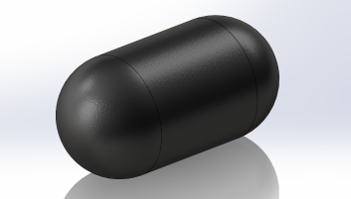
\includegraphics[width=\textwidth]{figures/chap3/payload_container_full.png}
        \caption{Full view of the closed container.}
        \label{fig:payload_container_full}
    \end{subfigure}
    \begin{subfigure}[b]{0.3\textwidth}
        \centering
        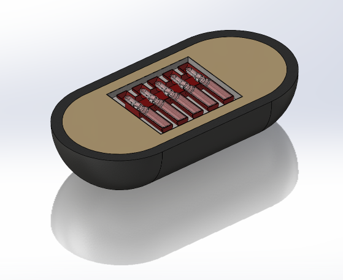
\includegraphics[width=\textwidth]{figures/chap3/payload_container_section.png}
        \caption{Sectioned view showing the outer shell, the foam filling, and the housed payload.}
        \label{fig:payload_container_section}
    \end{subfigure}
    \caption[Payload container geometry]{\hl{IT's REALLY UGLY}Payload container geometry: cylindrical central body capped with two hemispherical domes.}
    \label{fig:payload_container}
\end{figure}

Due to the artisanal nature of this design, linked to the difficulty in modelling specific 3D-printed PETG and the unquantifiable specifications of the insulation material, the payload container was modelled by retaining its shape with a 5 mm thick shell [\hl{verify thickness in the FE model}] of injection-moulded Acrylonitrile butadiene styrene (ABS), commonly used in packaging. The cavity is filled with polyurethane foam, chosen to simulate a protective wrapping (such as bubble wrap) that medical operators would use as established praxis to mitigate vibrations. The thermal paint is omitted from the payload container modelling process.



\subsubsection{Payload}
Considering the wide variety of medical goods potentially suitable for UAV-based air transport, it was necessary to identify a payload representative of standard shipments, excluding human organs and specialized equipment (e.g. defibrillators) to focus specifically on pharmaceuticals. Therefore, glass phials of the medicinal product \textit{Akineton Fiale}, containing \textit{biperidene lactate} at a concentration of 5\,mg/ml in injectable solution and shown in Fig.\ref{fig:akineton}\footnote{Source of photo: \url{https://www.guttafarm.net/akineton-cena}.}, were chosen. The product is commercially supplied in boxes of five phials, each individually packaged in a plastic blister tray.

\begin{figure}[h!]
    \centering
    \begin{subfigure}[b]{0.25\textwidth}
        \centering
        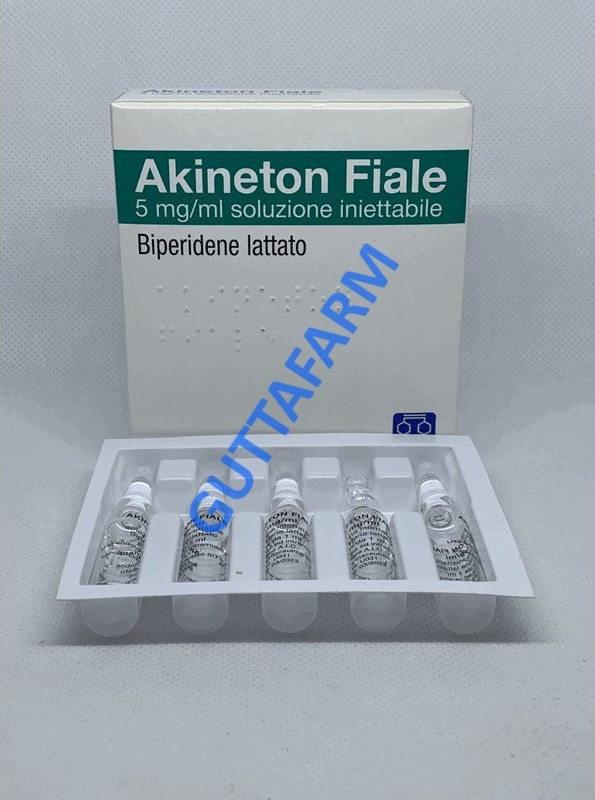
\includegraphics[width=\textwidth]{figures/chap3/akineton_fiale.jpg}
        \caption{Akineton Fiale, 5\,mg/ml injectable solution, as supplied in its original packaging.}
        \label{fig:akineton_box}
    \end{subfigure}
    \begin{subfigure}[b]{0.37\textwidth}
        \centering
        \includegraphics[width=\textwidth]{example-image-b}
        \caption{\hl{Single Akineton phial.}}
        \label{fig:akineton_phial}
    \end{subfigure}
    \caption{Akineton Fiale packaging and single phial.}
    \label{fig:akineton}
\end{figure}

Akineton is a pharmaceutical product commonly used in the treatment of Parkinson's disease and drug-induced extrapyramidal symptoms, and is usually administered by intravenous or intramuscular injection. For the purposes of the present thesis, only the mechanical properties of the glass container are of interest, as the pharmacological action of the medical fluid is not relevant to the type of structural analyses implemented in this study.


\subsection{Information gap}
The only missing inputs required for a full design workflow evaluation are:
\begin{itemize}
    \item The derived \textit{impact velocity}, angle, and mass for the selected scenario;
    \item The quantification of the phials' fragility through the characterisation of their material's mechanical \textit{allowables};
\end{itemize}

These failure scenario data must be fed into the design loop(s) proposed below to enable an effective design of the airbag-based impact attenuation system.

\section{Proposed approach}\label{section:proposed-approach}
\subsection{Outer design loop: formalising the \textit{Safety-First} principle}\label{section:outer-design-loop}

In response to the gap identified in Section \ref{section:payload-first-approach}, the first cotribution of this thesis is to propose an alternative design approach adopting (and later testing) the following guidelines:

\begin{objectivebox}[colframe=green!45!black, colback=green!60!black!8]{\textit{Safety-First} Design Principle}
\begin{enumerate}
\item The airframe and payload must be considered as two distinct entities;
\item In the type of operations considered, saving the payload takes higher priority than saving the airframe (carrying organs, expensive vaccines, emergency medicines, or high-value medical equipment is worth more than the drone itself);
\item Overall, the objectives are to minimise or mitigate:
    \begin{itemize}
    \item ground impact consequences,
    \item payload damage (preserving its integrity),
    \item environmental dispersion;
    \end{itemize}
\item These considerations should be applied at the beginning of the design process, possibly by integrating multiple safety devices (e.g., an airbag and a parachute working in tandem) and adjusting flight-mechanics considerations accordingly.
\end{enumerate}
\end{objectivebox}

A direct consequence of applying the Safety-First design principle in UAV-based operations' design is changing the sequence of design events, as exemplified in the simple flowcharts of Fig. \ref{fig:flowcharts-mission-vs-safety}, where Fig. \ref{fig:flowchart-mission-first} and Fig. \ref{fig:flowchart-safety-first} compare scenarios in which the mission loop can be interchanged with the safety loop to achieve design convergence. 


\begin{figure}[!htb]
    \centering
    \begin{subfigure}[t]{0.3\textwidth}
        \centering
        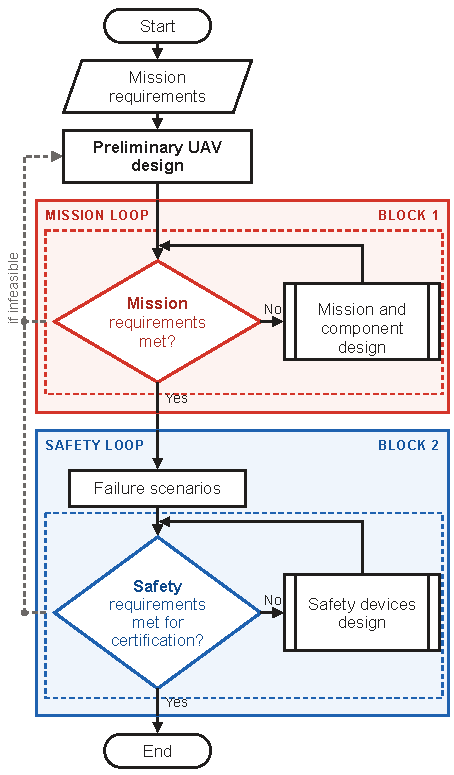
\includegraphics[width=\textwidth]{figures/chap3/flowchart-mission-first.pdf}
        \caption{\textit{Mission-First} approach}
        \label{fig:flowchart-mission-first}
    \end{subfigure}
    \hspace{0.08\textwidth}
    \begin{subfigure}[t]{0.3\textwidth}
        \centering
        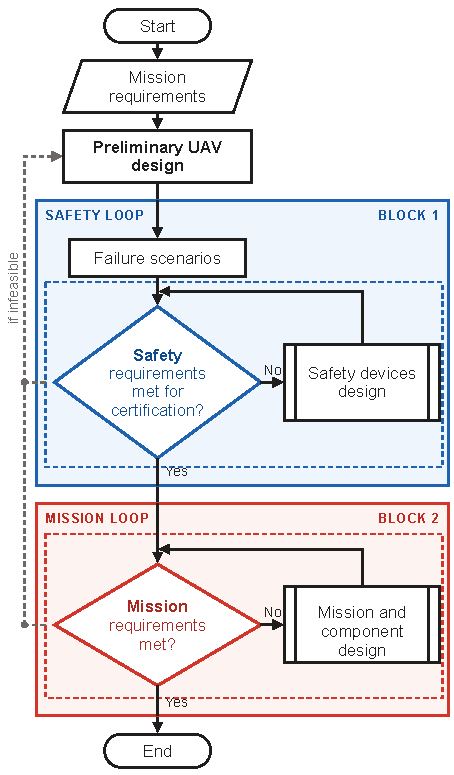
\includegraphics[width=\textwidth]{figures/chap3/flowchart-safety-first.pdf}
        \caption{\textit{Safety-First} approach}
        \label{fig:flowchart-safety-first}
    \end{subfigure}
    \caption{Sequence of design events in the two approaches: \textit{mission-first} and \textit{safety-first} loops.}
    \label{fig:flowcharts-mission-vs-safety}
\end{figure}



\subsection{Inner design loop: a payload-protection subsystem design workflow}\label{section:inner-design-loop}
This section aims to expand the \textit{Safety loop} concept presented in Section \ref{section:outer-design-loop} by informing it with the design guidelines distilled in Section \ref{section:airbag-design-guidelines}. The proposed workflow can be seen in Fig. \ref{fig:inner-design-loop}, and is divided into seven steps that bridge the gap between payload allowables' evaluation and safety device (airbag) prototyping. The loop is also split into two main branches, highlighting the boundary between the present MSc Thesis' deliverable and steps left to future developers. The first branch (steps 0-4) is partially payload-specific, meaning that some of the considerations made throughout these steps depend on the specific medical payload considered, while also generalisable to a broader spectrum of medical payload receptacles; the second branch (steps 5-7) are exclusively geometry-specific, implying that they require information on receptacle design, UAV-container hooking mechanism, and general information on system bulk, making them unattainable for the DIMEAS feasibility studies group, as they currently lack access to a functional medical payload container beyond their initial artisanal prototype by \cite{Sivieri2021}. Completing the workflow should lead directly to the \text{Mission loop} as shown earlier in Section \ref{section:outer-design-loop}.

\begin{figure}[!htb]
    \centering
    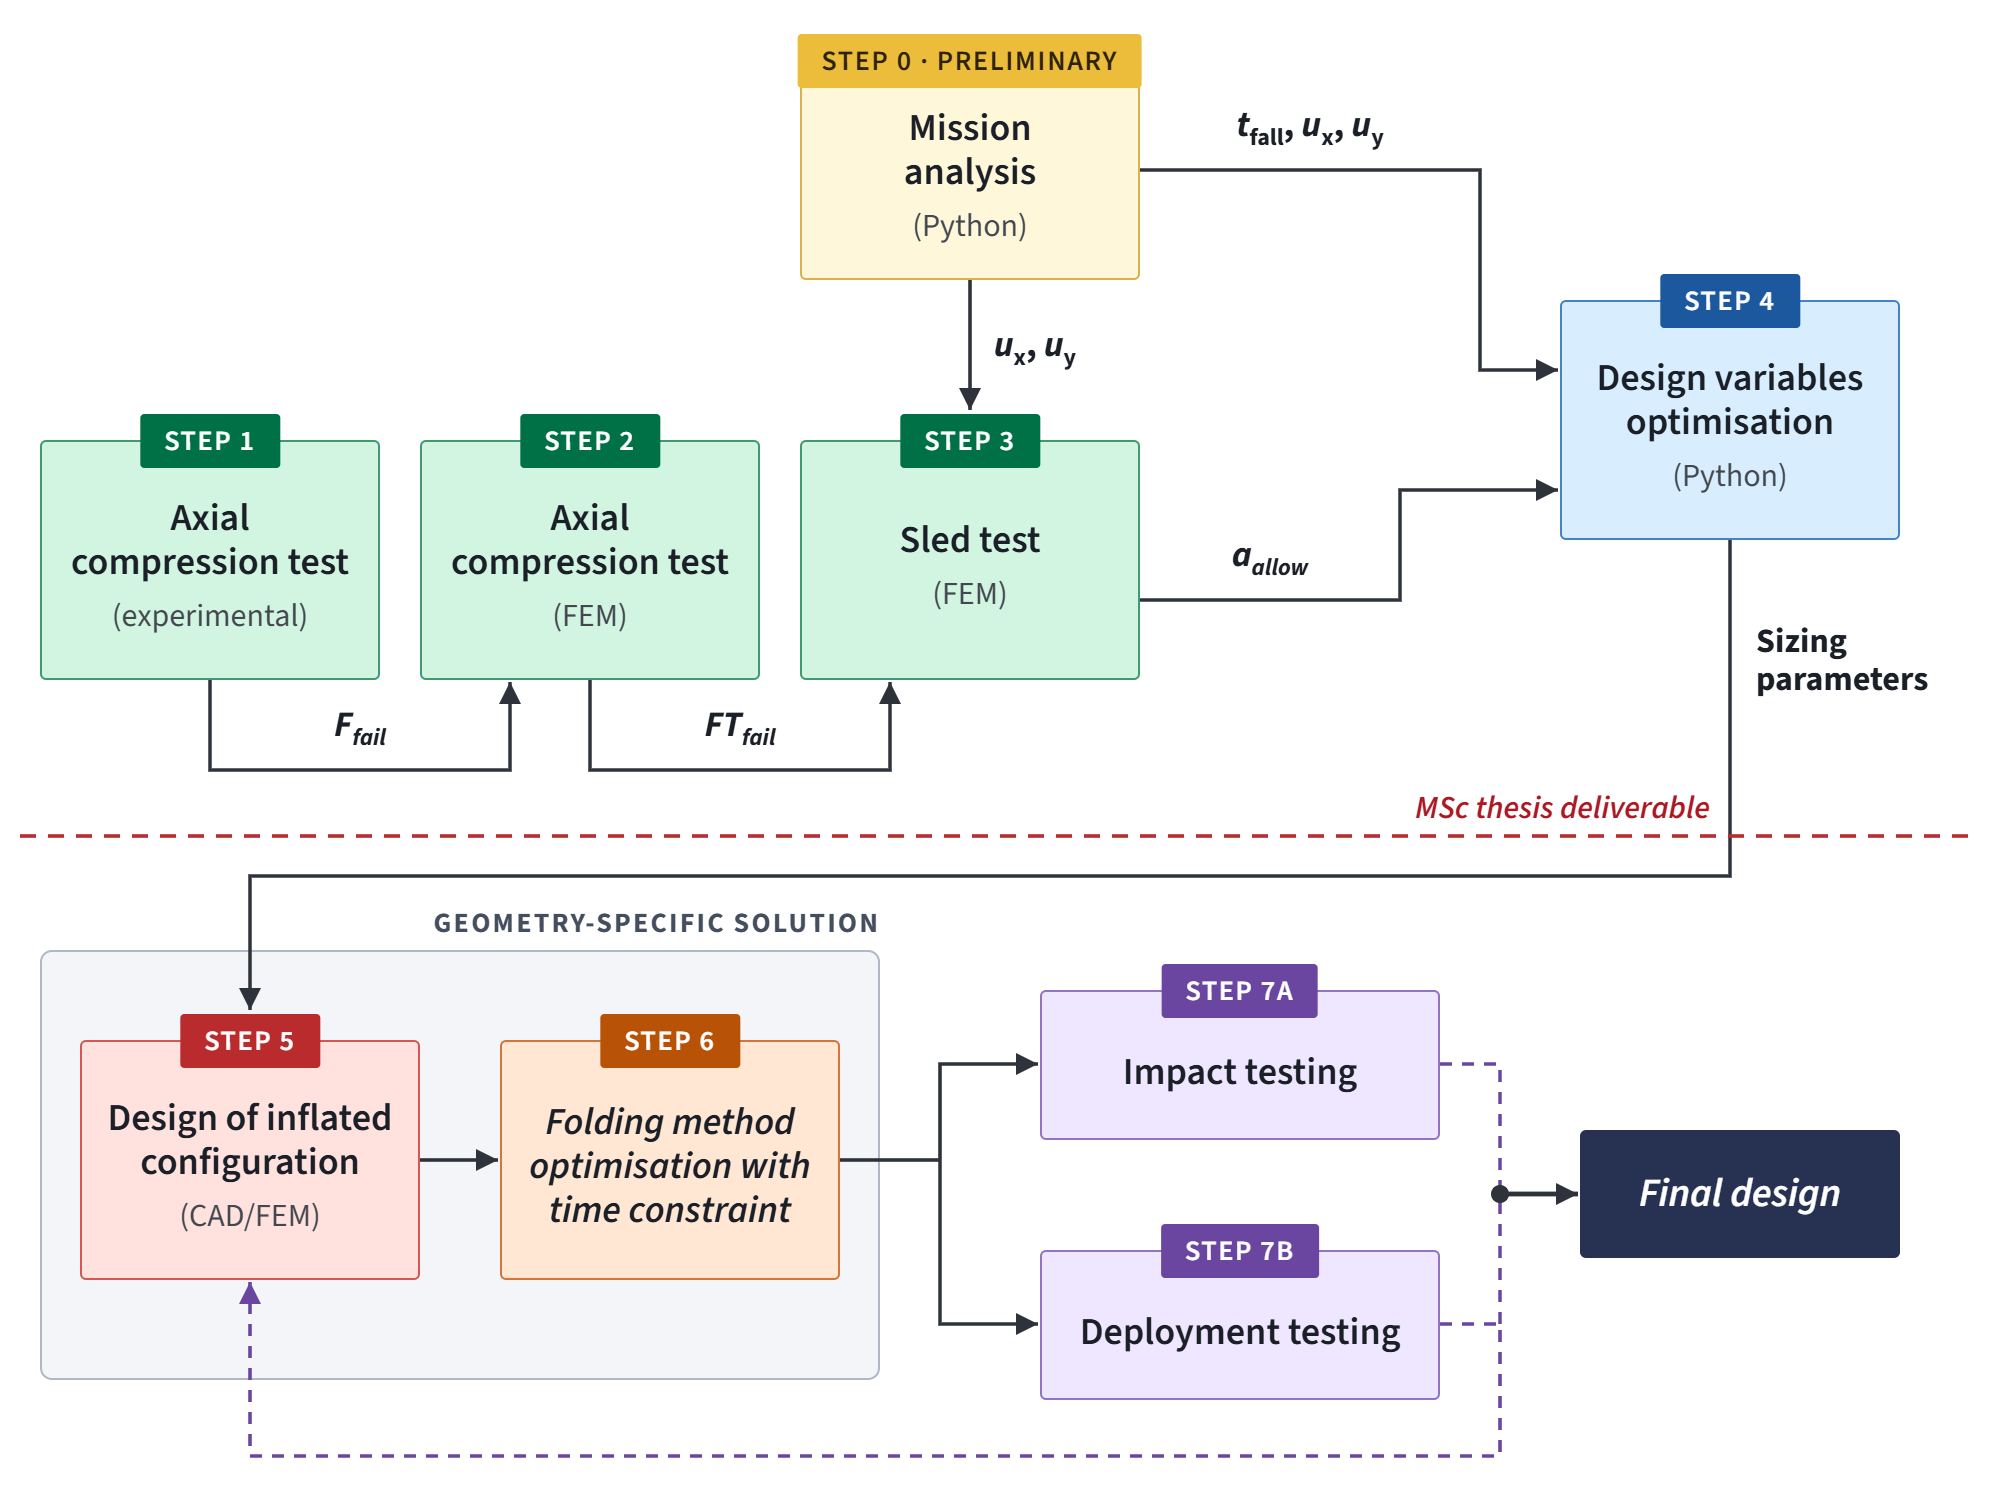
\includegraphics[width=0.85\textwidth]{figures/chap3/inner_loop_2-rows.png}
    \caption{Inner design loop, specific for the airbag-based payload-protection subsystem.}
    \label{fig:inner-design-loop}
\end{figure}


\subsubsection{Step 0 - Preliminary mission analysis}
This step covers the preliminary analysis of the payload's impact conditions. It evaluates the drop scenario, incorporates statistical analysis of wind direction and cruising conditions, and computes the trajectory and landing location of the payload. Serving as a general free-fall analysis, this phase yields key design inputs: the free-fall time ($t_{\text{fall}}$) and the horizontal and vertical impact velocities ($V_x$, $V_y$ respectively).

\subsubsection{Step 1 - Axial compression test (experimental)}
This step covers the experimental characterisation of the glass phials' (the selected medical payload) breaking point through laboratory testing. The goal is to conduct a test campaign to characterise the phial's mechanical behaviour, specifically providing key data, such as the failure force ($F_{\text{fail}}$, better defined in Section \ref{section:step1-test}), which feeds into the next phase to accurately calibrate the Finite Element Method (FEM) model.

\subsubsection{Step 2 - Axial compression test (FEM)}
This step focuses on matching the experimental behaviour observed in Step 1 with a Finite Element Method (FEM) model to accurately reproduce the material's mechanical response. Specifically, both experimentally and in the FEM model, the phials are subjected to axial compression loads, resembling the stress type to which they would be subjected to during an impact event. To replicate the laboratory results and build a calibrated material card that captures the phial's failure behaviour, the simulation mirrors the physical testing setup as closely as possible. This yields a generally realistic phial model, complete with its brittle failure threshold ($FT_{\text{fail}}$), that can be integrated into the full sled-test impact simulation in Step 3.

\subsubsection{Step 3 - Sled test}
This step involves simulating a sled test, heavily inspired by automotive industry practices, to observe the mechanical response of a test article (such as a dummy in vehicle crash testing, or in this case, a glass phial) measured through perceived accelerations and damage under an input acceleration profile. The simulated test subjects the payload container (based on the artisanal design proposed by \cite{Sivieri2021}) to realistic impact scenarios by reproducing an acceleration profile equivalent to a free-fall impact under the conditions defined in Step 0. This approach relies on the principle that the accelerations experienced by the payload directly correlate with the kinetic energy that must be dissipated during impact, linking the input acceleration profile to the resulting output. The primary output of this phase is the payload's allowable acceleration ($a_{\text{allow}}$).

\subsubsection{Step 4 - Design variables optimisation}
This fourth and final step of the thesis deliverable translates the established boundary conditions evaluated in previous steps (failure loads, allowable peak accelerations, impact velocities) into a numerical Python script for airbag sizing. Building upon the framework established in Section 2.1, the simulation optimises the airbag design against critical criteria, including total mass, bottoming-out speed, and rebound behaviour. Ultimately, this tool yields fundamental sizing parameters that will inform the future geometry-specific design of the system.


\subsubsection{Steps 5-7: Design of inflated configuration, folding method optimisation, impact and deployment testing}
Steps 5 and 6 shift the focus to geometry-specific development. Step 5 details the fully inflated configuration tailored directly to the geometry of the payload and UAV, matching the gas generator mechanism to the drone layout and impact timelines. Step 6 then builds upon this complete configuration by incorporating real-world manufacturing constraints, such as folding patterns, seaming details, and stowage volume, to optimise the deployment mechanism. While inherently interconnected, Step 6 specifically targets deployment time optimisation, as defined in Table \ref{tab:variable_inventory}.

Once a preliminary design and folding mechanism are established, the prototype undergoes a two-part experimental validation campaign: Step 7A (deployment testing) and Step 7B (impact testing). This phase validates the FEM models of steps 5 and 6 by subjecting physical prototypes to real-world impact conditions, operating in an iterative feedback loop between simulation and testing until design convergence is achieved.
